\documentclass[a4paper]{article}
\usepackage[spanish]{babel}
\usepackage[utf8]{inputenc}
\usepackage{fancyhdr}
\usepackage{charter} % tipografia
%\usepackage{graphicx}
\usepackage[pdftex]{graphicx}
\usepackage{bm} % bold font in math mode
\usepackage{sidecap}
\usepackage{caption}
\usepackage{subcaption}
\usepackage{booktabs}
\usepackage{makeidx}
\usepackage{float}
\usepackage{amsmath, amsthm, amssymb}
\newtheorem{theorem}{Teorema}
\newtheorem{customthm}{Teorema}
\newtheorem{corollary}{Corolario}[theorem]
\newtheorem{proposition}[theorem]{Proposición}
\newtheorem{innercustomlemma}{Lemma}
\newenvironment{customlemma}[1]
  {\renewcommand\theinnercustomlemma{#1}\innercustomlemma}
  {\endinnercustomlemma}
\usepackage{amsfonts}
\usepackage{sectsty}
\usepackage{wrapfig}
\usepackage{listings}
\usepackage{hyperref} % links
\usepackage{algorithm} %http://www.ctan.org/pkg/algorithms
\usepackage{algorithmic}
\usepackage[usenames,dvipsnames]{xcolor}
\usepackage{pgfplots}
\usepackage{tabularx} % tablas copadas
% \usepackage{pgfplotstable}
% custom
\usepackage{color} % para snipets de codigo coloreados
\usepackage{fancybox} % para el sbox de los snipets de codigo
\definecolor{litegrey}{gray}{0.94}
% \newenvironment{sidebar}{%
% \begin{Sbox}\begin{minipage}{.85\textwidth}}%
% {\end{minipage}\end{Sbox}%
% \begin{center}\setlength{\fboxsep}{6pt}%
% \shadowbox{\TheSbox}\end{center}}
% \newenvironment{warning}{%
% \begin{Sbox}\begin{minipage}{.85\textwidth}\sffamily\lite\small\RaggedRight}%
% {\end{minipage}\end{Sbox}%
% \begin{center}\setlength{\fboxsep}{6pt}%
% \colorbox{litegrey}{\TheSbox}\end{center}}

%\newenvironment{codesnippet}{%
%\begin{Sbox}\begin{minipage}{\linewidth-2\fboxsep-2\fboxrule-4pt}\sffamily\small}%
%{\end{minipage}\end{Sbox}%
%\begin{center}%
%\colorbox{litegrey}{\TheSbox}\end{center}}

% \newenvironment{codesnippet}{\VerbatimEnvironment%
%   \noindent
%   %{\columnwidth-\leftmargin-\rightmargin-2\fboxsep-2\fboxrule-4pt}
%   \begin{Sbox}
%   \begin{minipage}{\linewidth-2\fboxsep-2\fboxrule-4pt}
%   \begin{Verbatim}
% }{%
%   \end{Verbatim}
%   \end{minipage}
%   \end{Sbox}%
%   \colorbox{litegrey}{\TheSbox}
% }

\newenvironment{codesnippet}{%
  \noindent
  %      {\columnwidth-\leftmargin-\rightmargin-2\fboxsep-2\fboxrule-4pt}
  \begin{Sbox}
  \begin{minipage}{\linewidth}
  \begin{lstlisting}
}{
  \end{lstlisting}
  \end{minipage}
  \end{Sbox}%
  \colorbox{litegrey}{\TheSbox}
}

\usepackage{fancyhdr}
\pagestyle{fancy}
%\renewcommand{\chaptermark}[1]{\markboth{#1}{}}
\renewcommand{\sectionmark}[1]{\markright{\thesection\ - #1}}
\fancyhf{}
\fancyhead[LO]{Sección \rightmark} % \thesection\
\fancyfoot[LO]{\small{Iv\'an Arcuschin, Mart\'in Jedwabny, Jos\'e Massigoge, Iv\'an Pondal}}
\fancyfoot[RO]{\thepage}
\renewcommand{\headrulewidth}{0.5pt}
\renewcommand{\footrulewidth}{0.5pt}
\setlength{\hoffset}{-0.8in}
\setlength{\textwidth}{16cm}
%\setlength{\hoffset}{-1.1cm}
%\setlength{\textwidth}{16cm}
\setlength{\headsep}{0.5cm}
\setlength{\textheight}{25cm}
\setlength{\voffset}{-0.7in}
\setlength{\headwidth}{\textwidth}
\setlength{\headheight}{13.1pt}
\renewcommand{\baselinestretch}{1.1} % line spacing

% -------------------- COMANDOS ESPECIALES ------------------------------

\newcommand{\calcular}[2]{\pgfmathtruncatemacro{#1}{#2}}

\pgfplotsset{
  filter params/.style n args={4}{
      x filter/.code={
          \edef\tempa{\thisrow{#1}}
          \edef\tempb{#2}
          \edef\tempc{\thisrow{#3}}
          \edef\tempd{#4}
          \ifx\tempa\tempb
            \ifx\tempc\tempd
            \else
              \def\pgfmathresult{inf}
            \fi
          \else
            \def\pgfmathresult{inf}
          \fi
      }
  }
}

\newcommand{\graficarDatos}[6]{
  \begin{tikzpicture}
  \begin{axis}[
      title={#1},
      xlabel={#2},
      ylabel={#3},
      scaled x ticks=false,
      scaled y ticks=false,
      scale=0.5
  ]
  \addplot[only marks, color=black] table[x=#4,y=#5]{#6};
  \end{axis}
  \end{tikzpicture}
}

\newcommand{\graficarDatosPlus}[7]{
  \begin{tikzpicture}
  \begin{axis}[
      title={#1},
      xlabel={#2},
      ylabel={#3},
      scaled x ticks=false,
      scaled y ticks=false,
      width=0.6\textwidth,
      #7
  ]
  \addplot[only marks, color=black] table[x=#4,y=#5]{#6};
  \end{axis}
  \end{tikzpicture}
}

\makeatletter
\pgfplotsset{
    groupplot xlabel/.initial={},
    every groupplot x label/.style={
        at={($({group c1r\pgfplots@group@rows.west}|-{group c1r\pgfplots@group@rows.outer south})!0.5!({group c\pgfplots@group@columns r\pgfplots@group@rows.east}|-{group c\pgfplots@group@columns r\pgfplots@group@rows.outer south})$)},
        anchor=north,
    },
    groupplot ylabel/.initial={},
    every groupplot y label/.style={
            rotate=90,
        at={($({group c1r1.north}-|{group c1r1.outer
west})!0.5!({group c1r\pgfplots@group@rows.south}-|{group c1r\pgfplots@group@rows.outer west})$)},
        anchor=south
    },
    execute at end groupplot/.code={%
      \node [/pgfplots/every groupplot x label]
{\pgfkeysvalueof{/pgfplots/groupplot xlabel}};
      \node [/pgfplots/every groupplot y label]
{\pgfkeysvalueof{/pgfplots/groupplot ylabel}};
    },
    group/only outer labels/.style =
{
group/every plot/.code = {%
    \ifnum\pgfplots@group@current@row=\pgfplots@group@rows\else%
        \pgfkeys{xticklabels = {}, xlabel = {}}\fi%
    \ifnum\pgfplots@group@current@column=1\else%
        \pgfkeys{yticklabels = {}, ylabel = {}}\fi%
}
}
}

\def\endpgfplots@environment@groupplot{%
    \endpgfplots@environment@opt%
    \pgfkeys{/pgfplots/execute at end groupplot}%
    \endgroup%
}
\makeatother

\newcommand{\barGraphExp}[2]{
    \begin{tikzpicture}
    \begin{axis}[
        xlabel={Implementación},
    	ylabel={Tiempo de ejecución (clocks)},
        legend style={at={(1.4,1.0)}},
        ybar,
        scaled ticks=false,
        width=0.5\textwidth,
        height=0.5\textwidth,
        tickpos=left,
        xtick=\empty,
        ytick align=inside,
        xtick align=inside,
    	enlargelimits=0.05,
        bar width=16,
    ]
    % How to process each item:
    \renewcommand*{\do}[1]{\addplot+[color=black] table[x=n, y=##1]{datos/datos_blur.dat};}
    % Process list:
    \docsvlist{#2}
    \legend{#2}
    \end{axis}
    \end{tikzpicture}
}

\newcommand{\graficarDatosExp}[6]{
  \begin{tikzpicture}
  \begin{axis}[
      title={#1},
      xlabel={#2},
      ylabel={#3},
      scaled x ticks=false,
      scaled y ticks=false,
      enlargelimits=0.05,
      width=0.5\textwidth,
      height=0.5\textwidth
  ]
  \addplot[color=black] table[x=#5,y=#6]{#4};
  % \renewcommand*{\do}[1]{\addplot table[x=#5,y=##1]{#4};}
  % %     % Process list:
  % \docsvlist{#6}
  % \legend{#6}
  \end{axis}
  \end{tikzpicture}
}

% ------------------------------------------------------------------------

% \setcounter{secnumdepth}{2}
\usepackage{underscore}
\usepackage{kbordermatrix}% Matrix column labels
\usetikzlibrary{arrows,shapes}
\usepackage{tkz-graph}
\usepackage{caratula}
\usepackage{url}
\lstset{
    language=C++,
    basicstyle=\ttfamily,
    keywordstyle=\color{blue}\ttfamily,
    stringstyle=\color{red}\ttfamily,
    commentstyle=\color{ForestGreen}\ttfamily,
    morecomment=[l][\color{magenta}]{\#},
    literate={á}{{\'a}}1 {ó}{{\'o}}1 {é}{{\'e}}1 {í}{{\'i}}1 {ú}{{\'u}}1 {Á}{{\'A}}1 {Í}{{\'I}}1 {É}{{\'E}}1 {Ú}{{\'U}}1 {Ó}{{\'O}}1 {\ \ }{{\ }}1,
	breaklines=true,
	tabsize=2
}

\DeclareUnicodeCharacter{2212}{-}

% *********************** %
\usepackage{tikz}
\usetikzlibrary{graphs}
\usetikzlibrary{calc}
\usetikzlibrary{arrows}
\usetikzlibrary{matrix}
% Otros
\usepackage{arrayjobx}
\usepackage{enumitem}
\usepackage{multicol}
\usepackage{natbib}
\usepackage{etoolbox}
\usepackage{listingsutf8}
\lstset{inputencoding=utf8/latin1}
\usepackage{fancyvrb}
\usepackage{pgfplotstable}
\usepackage{float}
\newcommand{\subscript}[2]{$#1 _ #2$}


% ******************************************************** %
\begin{document}
\thispagestyle{empty}
\materia{Teoría de las Comunicaciones}
\submateria{Primer Cuatrimestre de 2016}
\titulo{Trabajo Práctico I}
%\subtitulo{Grupo: }
\integrante{Iv\'an Arcuschin}{678/13}{iarcuschin@gmail.com}
\integrante{Federico De Rocco}{408/13}{fede.183@hotmail.com}
\integrante{Mart\'in Jedwabny}{885/13}{martiniedva@gmail.com}
\integrante{Jos\'e Massigoge}{954/12}{jmmassigoge@gmail.com}
\maketitle
% no footer on the first page
\thispagestyle{empty}
\newpage

\tableofcontents

\newpage
\section{Introducción}
En este trabajo práctico nos proponemos analizar redes de información con el objetivo de puntualizar diversos aspectos analíticos de las mismas. Para lograr tal fin, desarrolamos una herramienta a partir de la librería \textit{Scapy}, la cual nos provee de una función llamada \texttt{sniff} y el software Wireshark. Ambos nos permitieron capturar todos los paquetes visibles de la red en la cual nos encontramos durante un período de tiempo determinado.

Basándonos en la teoría de la información de Shannon y con los paquetes obtenidos, definimos tres fuente de información, $S$, $S_{1}$ y $S_{2}$, donde:

\begin{itemize}
  \item $S = \{s_{1} \dots s_{n}\}$, donde $s_{i}$ es el valor del campo \emph{type} de cada paquete \texttt{Ethernet} de capa 2.
  \item $S_{1} = \{s_{1} \dots s_{n}\} $, donde $s_i$ es el valor del campo \emph{destino} (IP) de cada paquete de
  tipo \texttt{ARP} Who-Has.
\end{itemize}

Es necesario aclarar que los paquetes \texttt{ARP}, el cual es un protocolo de capa 2.5, se utilizan para encontrar direcciones \texttt{MAC} (direcciones de capa 2) asociadas a cada \texttt{IP} (direcciones de capa 3). El procedimiento por el cual un host envía un paquete \texttt{ARP} se inicia cuando el host quiere enviar un paquete a una dirección IP, la cual se encuentra dentro de su red local, y no esta listada dentro de su tabla de traducciones de direcciones \texttt{MAC-IP}. Luego el host envía un paquete \texttt{ARP} de tipo Who-Has broadcast, dentro de su red local, para determinar la dirección \texttt{MAC} del host destino. El host con la dirección \texttt{IP} solicitada responde únicamente al host fuente con su dirección \texttt{MAC}, utilizando un paquete \texttt{ARP} de tipo Is-At.

A partir de la definición de las fuentes, lo que nos importa es determinar la cantidad de información $I(s_{i}) = -log_2(P(s_{i}))$ que aporta cada símbolo de la fuente, donde $Ps_{i}$ es la probabilidad de ocurrencia del símbolo $s_{i}$, la cual se obtiene mediante el cociente entre la cantidad de apariciones de $s_{i}$ en los paquetes y la cantidad total de paquetes capturados.

Luego vamos a comparar cada $I(s_{i})$ con la entropía de la fuente, $H(S_{i}) = \sum\limits_{s \in S_{i}} P(s) * I(s)$, para observar la presencia de \emph{protocolos distinguidos}, en el caso de la fuente $S$, o \emph{nodos distinguidos}, en el caso de la fuente $S_{1}$ y $S_{2}$. La noción de elemento distinguido la definimos como aquel símbolo cuya información es menor a la entropía de la fuente, es decir que la cantidad de información que aporta ese símbolo es baja, ya que el símbolo es predecible. La finalidad de este análisis parte de la idea de que una fuente cualquiera, $S$, sin perdida de información, satisface la ecuación $H(S) \leq L(C)$, donde $L(C)$ es el largo de la codificación $C$ de los símbolos de $S$. Para lograr que la codificación $C$ sea óptima, debemos codificar los símbolos distinguidos con menos bits que el resto de los símbolos de la fuente. Este tipo de análisis nos permite determinar que tan comprensible es una fuente, ya que cuanto menor sea su entropía mayor es su capacidad de comprensión.

Otro aspecto que vamos a analizar de las redes de información es la incidencia de los paquetes \texttt{ARP} en las mismas. Dado que estos paquetes son de control, es decir no transportan datos, impactan negativamente en el $throughput$ de una red, siendo $throughput$ el volumen de información neta que fluye a través de una red. Este análisis nos permitirá definir que red es mas eficiente en términos de datos transportados.


\newpage
\section{Experimentos}
%En esta sección desarrollaremos y mostraremos los resultados de los experimentos para:

\begin{itemize}
\item Los protocolos distinguidos.
\item La incidencia de paquetes ARP en la red.
\item Los nodos distinguidos.
\end{itemize}

\subsection{Experimento protocolos distinguidos}

Para analizar los protocolos distinguidos fuimos guardando los resultados de sniffear diferentes redes y tomar como fuente de información S el campo .type de los paquetes que se fueron procesando. Fundamentalmente vimos tres tipos de protocolos: ARP, IP (es decir IPv4) e IPv6. Dentro de los paquetes IP pudimos ver que la mayoría, a su vez, llevaban paquetes ICMP, TCP o UDP. A traves de la libreria "Scapy" de "Python" tomamos dos muestras de los paquetes 'Ethernet' que se pudieron detectar:

\begin{itemize}
\item Dataset 1: Biblioteca pabellón 2 (wifi) a las 3pm
\item Dataset 2: Laboratorios pabellón 1 (wifi) a las 5pm
\end{itemize}

Cada dataset contiene todos los paquetes observados junto al protocolo que se uso. De ahí calculamos la cantidad de apariciones de cada protocolo, la probabilidad de aparición de cada protocolo, calculamos la entropía y la comparamos con la información que aporta cada símbolo de S (ARP, IP e IPv6).\\

Por eso, para distinguir \emph{protocolos} tomamos a
aquellos cuya probabilidad de aparición era alta, de forma que la información provista por el símbolo fuera menor a la entropía de la fuente S.\\

Ahora, para analizar los datos, planteamos histogramas donde podemos ver la cantidad de información $I(s) = -log_2(P(s))$ que aporta cada símbolo de la fuente. Luego lo comparamos con la entropía y definimos los \emph{protocolos distinguidos} como los que son mas bajos que la entropía. Esto lo hicimos porque según la fórmula de Shannon, la entropía $\sum\limits_{s \in S} P(s) * I(s)$ se corresponde con la información promedio que aporta cada símbolo a la fuente. Por lo cual, los símbolos cuya cantidad de información sea mas baja que la entropía son muy predecibles ya que aparecerán muchas veces y, por ejemplo, si tuviera que asignarle otro símbolo a cada uno de ellos, me convendría representarlos con menos bits para disminuir la longitud promedio del código. \\

Los resultados fueron los siguientes: \\

% Dataset 1 ----------------------------------

\begin{tikzpicture}
\begin{axis}[
    ybar,
    bar width=1cm, % Width of the bar
    x=1.5cm, % Distance between the centers of the bars
    enlarge x limits={abs=1cm}, % The distance between the center of the first bar and the left edge
    enlarge y limits=false,
    ymin=0,
    xtick=data,
    xlabel= {Dataset 1},
    ylabel= {Probabilidad},
    symbolic x coords={IPv6,ARP,IP},
    point meta={y*100}, %y-Werte mal 100 für Prozent 
    yticklabel={\pgfmathparse{\tick*100}\pgfmathprintnumber{\pgfmathresult}\%},
    axis lines*=left,
    clip=false
    ]
\addplot [
    draw=black,
    fill=white,
    nodes near coords={\pgfmathprintnumber{\pgfplotspointmeta}\,\%},
    error bars/.cd,
        y dir=both,
        y explicit
    ] coordinates{(IPv6,0.001998001998)
        (ARP,0.0679320679321)
        (IP,0.93006993007)};
\end{axis}
\end{tikzpicture}
\begin{tikzpicture}
\begin{axis}[
    symbolic x coords={IPv6,ARP,IP},
        ylabel = {Informacion del simbolo},
        xlabel = {Dataset 1},
        xtick=data]
    \addplot[ybar,fill=white] coordinates {
        (IPv6,8.9672262584)
        (ARP,3.8797634179)
        (IP,0.1045889014)
    };
    \draw [red] ({rel axis cs:0,0}|-{axis cs:ARP,0.378751880122}) -- ({rel axis cs:1,0}|-{axis cs:ARP,0.378751880122}) node [pos=0.33, above] {Entropia};
\end{axis}
\end{tikzpicture} \\

% Dataset 2 ----------------------------------

\begin{tikzpicture}
\begin{axis}[
    ybar,
    bar width=1cm, % Width of the bar
    x=1.5cm, % Distance between the centers of the bars
    enlarge x limits={abs=1cm}, % The distance between the center of the first bar and the left edge
    enlarge y limits=false,
    ymin=0,
    xtick=data,
    xlabel= {Dataset 2},
    ylabel= {Probabilidad},
    symbolic x coords={IPv6,ARP,IP},
    point meta={y*100}, %y-Werte mal 100 für Prozent 
    yticklabel={\pgfmathparse{\tick*100}\pgfmathprintnumber{\pgfmathresult}\%},
    axis lines*=left,
    clip=false
    ]
\addplot [
    draw=black,
    fill=white,
    nodes near coords={\pgfmathprintnumber{\pgfplotspointmeta}\,\%},
    error bars/.cd,
        y dir=both,
        y explicit
    ] coordinates{
        (IPv6,0.1389218889)
        (ARP,0.3728838729)
        (IP,0.4881942382)};
\end{axis}
\end{tikzpicture}
\begin{tikzpicture}
\begin{axis}[
    symbolic x coords={IPv6,ARP,IP},
        ylabel = {Informacion del simbolo},
        xlabel = {Dataset 2},
        xtick=data]
    \addplot[ybar,fill=white] coordinates {
        (IPv6,2.847654163)
        (ARP,1.423201692)
        (IP,1.034472826)
    };
    \draw [red] ({rel axis cs:0,0}|-{axis cs:ARP,1.4313141279}) -- ({rel axis cs:1,0}|-{axis cs:ARP,1.4313141279}) node [pos=0.33, above] {Entropia};
\end{axis}
\end{tikzpicture} \\

% Discusion ------------------------------------

Por lo que podemos ver, la incidencia de ARP es muy baja en el Dataset 1 ya que en una biblioteca hay poco recambio de dispositivos y pocos hosts, lo cual hace que la incidencia de ARP sea menor. En cambio, si hay muchos mas paquetes IP, lo cual tiene sentido porque es el protocolo que todos los hosts usan para conectarse a internet. Entonces como podemos ver, el único símbolo predecible menor que la entropía es el de IP, el cual es el único protocolo distinguido en este dataset. \\

En el segundo Dataset, ya podemos hablar de una red (el Laboratorio de Computación) en la cual no solamente hay muchos mas hosts, sino el recambio de dispositivos que entran y se van de la red es mayor, por lo cual la incidencia de ARP sube. A su vez, IP sigue siendo el protocolo más usado al igual que en el dataset anterior. Tanto la información que aporta ARP como IP superan la entropía de la fuente de información S, por eso ambos son en este caso protocolos distinguidos. \\
% end subsection

\subsection{Experimento incidencia de ARP}

Usaremos la misma forma de medir que describimos en el ejercicio anterior para poder observar la incidencia de paquetes ARP en la red voy a utilizar una serie de muestras 
tomadas de distintas redes y graficarlas en un histograma, después de mostrar los resultados daremos una explicación del por que de los mismo. Aclaración: todas las capturas
son de 15 minutos.

\begin{figure}[ht!]
\centering
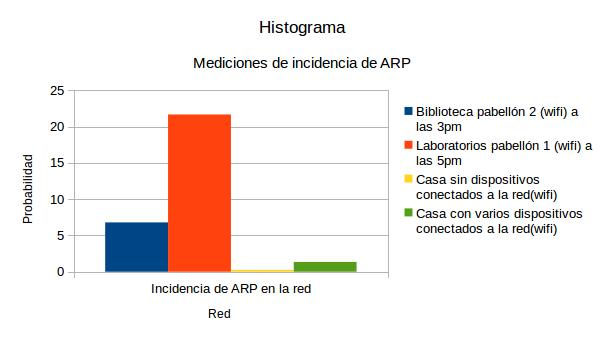
\includegraphics[width=90mm]{imagenes/IncidenciaARP.jpg}
\caption{Comparación de porcentaje de apariciones de ARP en distintas redes o con distintas condiciones.\label{overflow}}
\end{figure}

Como podemos ver la red de los laboratorios tiene más porcentaje de paquetes ARP que el de la biblioteca. Esto se debe a que en el laboratorio del pabellón 1 ingresan 
constantemente personas y, por lo tanto, la mayoría de ellos ingresan en la red a través de las computadoras del mismo o usando el wifi de estos con sus celulares. Esto 
ocurre en menor medida en la biblioteca ya que no se usan computadoras que no sean propias de los que ingresan, por lo tanto, hay mucho más tráfico de paquetes ARP en la red 
de los laboratorios. Además al estar en una red privada, es más común que se efectúen envíos de mensajes entre computadoras y los routers de las mismas.

En menor medida tenemos los casos tomados en la red de un hogar, teniendo como sus dos mediciones a cuando solamente hay un dispositivo, el mismo con el que se realiza la medición, 
conectado a la red y cuando hay más cantidad. Podemos ver que el tráfico de paquetes ARP es muy bajo en ambos casos en comparación a las muestras anteriores. Sin embargo, 
cuando hay mayor cantidad de dispositivos el tráfico general aumenta y también el porcentaje de paquetes ARP, porque en este caso hay mas hosts.

% end subsection

En esta sección desarrollaremos y mostraremos los resultados de los experimentos para:

\begin{itemize}
\item Los protocolos distinguidos.
\item La incidencia de paquetes ARP en la red.
\item Los nodos distinguidos.
\end{itemize}

Intento de experimentos1:

Para poder observar la incidencia de paqueres ARP en la red voy a utilizar el buscador de Google Chrome y la función de scapy arping. Usando la interfaz de wlan0 podre sniffear
los paquetes que habra con el buscador y usando arping podre enviar paquetes ARP.\\

Ejecuto  sudo ./capture.py wlan0 entropia-tipos 1000 y, al mismo tiempo, abro el buscador. 

Resultados:

Simbolo 2048 tiene probabilidad 0.996158770807(IP).

Simbolo 34525 tiene probabilidad 0.00128040973111(IPv6).

Simbolo 2054 tiene probabilidad 0.00256081946223(ARP).

La entropia de la fuente es 0.0492085855963.

Simbolo 2048 tiene probabilidad 0.996158770807(IP).

Simbolo 34525 tiene probabilidad 0.00256081946223(IPv6).

Simbolo 2054 tiene probabilidad 0.00128040973111(ARP).

La entropia de la fuente es 0.0398813035719.

Simbolo 2048 tiene probabilidad 0.99875(IP).

Simbolo 2054 tiene probabilidad 0.00125(ARP).

La entropia de la fuente es 0.0138570614629.

Simbolo 2048 tiene probabilidad 0.998740554156(IP).

Simbolo 2054 tiene probabilidad 0.00125944584383(ARP).

La entropia de la fuente es 0.013948087353.

Simbolo 2048 tiene probabilidad 0.985987261146(IP).

Simbolo 34525 tiene probabilidad 0.0101910828025(IPv6).

Simbolo 2054 tiene probabilidad 0.00382165605096(ARP).

La entropia de la fuente es 0.118197558737.

Ejecuto  sudo ./capture.py wlan0 entropia-tipos 100 y, al mismo tiempo, ejecuto arping("192.168.2.0/24").

Resultados:
Simbolo 2048 tiene probabilidad 0.0481481481481(IP).

Simbolo 2054 tiene probabilidad 0.951851851852(ARP).

La entropia de la fuente es 0.278477724908.

Simbolo 2048 tiene probabilidad 0.0769230769231(IP).

Simbolo 34525 tiene probabilidad 0.0244755244755(IPv6).

Simbolo 2054 tiene probabilidad 0.898601398601(ARP).

La entropia de la fuente es 0.554261234655.

Simbolo 2048 tiene probabilidad 0.0115384615385(IP).

Simbolo 2054 tiene probabilidad 0.988461538462(ARP).

La entropia de la fuente es 0.0908278259323.

Simbolo 2048 tiene probabilidad 0.011320754717(IP).

Simbolo 34525 tiene probabilidad 0.00754716981132(IPv6).

Simbolo 2054 tiene probabilidad 0.981132075472(ARP).

La entropia de la fuente es 0.153356025339.

Simbolo 2054 tiene probabilidad 1.0(ARP).

La entropia de la fuente es 0.0.

Ejecuto  sudo ./capture.py wlan0 entropia-tipos 100 y, al mismo tiempo, abro buscador y ejecuto arping("192.168.2.0/24").

Resultados:

Simbolo 2048 tiene probabilidad 0.737424547284(IP).

Simbolo 34525 tiene probabilidad 0.00201207243461(IPv6).

Simbolo 2054 tiene probabilidad 0.260563380282(ARP).

La entropia de la fuente es 0.847640262877.

Simbolo 2048 tiene probabilidad 0.735412474849(IP).

Simbolo 34525 tiene probabilidad 0.00603621730382(IPv6).

Simbolo 2054 tiene probabilidad 0.258551307847(ARP).

La entropia de la fuente es 0.875119992479.

Simbolo 2048 tiene probabilidad 0.761948529412(IP).

Simbolo 34525 tiene probabilidad 0.00183823529412(IPv6).

Simbolo 2054 tiene probabilidad 0.236213235294(ARP).

La entropia de la fuente es 0.807325191625.

Simbolo 2048 tiene probabilidad 0.757518796992(IP).

Simbolo 34525 tiene probabilidad 0.00093984962406(IPv6).

Simbolo 2054 tiene probabilidad 0.241541353383(ARP).

La entropia de la fuente es 0.808024777478.

Simbolo 2048 tiene probabilidad 0.754066985646(IP).

Simbolo 2054 tiene probabilidad 0.245933014354(ARP).

La entropia de la fuente es 0.804768238572.


Ejecuto  sudo ./capture.py wlan0 entropia-tipos 100 y, al mismo tiempo, arping("192.168.2.0/24") y arping("10.4.2.0/27").

\newpage
\section{Conclusiones}
En la introducción definimos dos fuentes de información $S$ y $S_{1}$, de las cuales, en la experimentación, calculamos su entropía y la información que provee cada símbolo. De esta manera pudimos distinguir determinados símbolos en cada fuente, según que Dataset utilizamos para el cálculo. A partir de ese cálculo, pudimos concluir que:
\begin{itemize}
  \item \textbf{Caso fuente $S$, protocolos}: Sin importar el Dataset, el protocolo \texttt{IP} se distingue claramente de los demás. Vale la pena mencionar el caso del protocolo \texttt{IPv6}, cuya probabilidad de ocurrencia es baja, lo cual da una pauta de su baja implementación.
  \item \textbf{Caso fuente $S_{1}$, nodos}: El Dataset juega un rol diferenciador a la hora de distinguir nodos, donde, según el Dataset, podemos observar uno o mas nodos distinguidos. Este fenómeno se explica por la topología de cada red, lo cual puede contener más de un gateway.
  Otra observación que se desprende sobre la topología de la redes es que su forma es de tipo estrella, lo cual condice con las metodologías de ruteo explicadas en clase.
\end{itemize}

Con respecto a la incidencia de los paquetes \texttt{ARP} en las diversas redes, pudimos observar que 
%existe una correlación entre la cantidad de nodos de la red y el porcentaje de paquetes \texttt{ARP}, siendo la misma proporcional. La razón de este fenómeno (especulamos) se debe a que, a mayor cantidad de nodos, mayor son los paquetes solicitando la dirección \texttt{MAC} del gateway y mayor es la probabilidad de que haya comunicaciones entre los diversos nodos de la red local. Dado que a mayor incidencia de paquetes \texttt{ARP} menor es el $throughput$, notamos un problema de escalabilidad de los protocolos vigentes, lo cual es producto de razones históricas, cuyo desenlace fue una proliferación de protocolos de capa 2, los cuales se buscaron homogeneizar con el protocolo \texttt{IP}, siendo necesario para tal fin, la introducción de los paquetes \texttt{ARP}. Entendemos que proponer/implementar otro protocolo de capa 2 y 3 es inviable y claramente escapa el alcance del presente trabajo.


% \newpage
% \bibliographystyle{plain}
% \section{Referencias}
% \begingroup
% \renewcommand{\section}[2]{}
% \bibliography{informe}
% \endgroup
%
% \newpage
% \appendix
% \input{apendice}

\end{document}
